
Um den Effekt der nebenläufigen Architektur möglichst zu isolieren, werden in den Szenarien 1 und 2 keine zufällig generierten Welten genutzt. Stattdessen werden die Blöcke nach einem festgelegten Muster gesetzt.

\begin{figure}
	\centering
	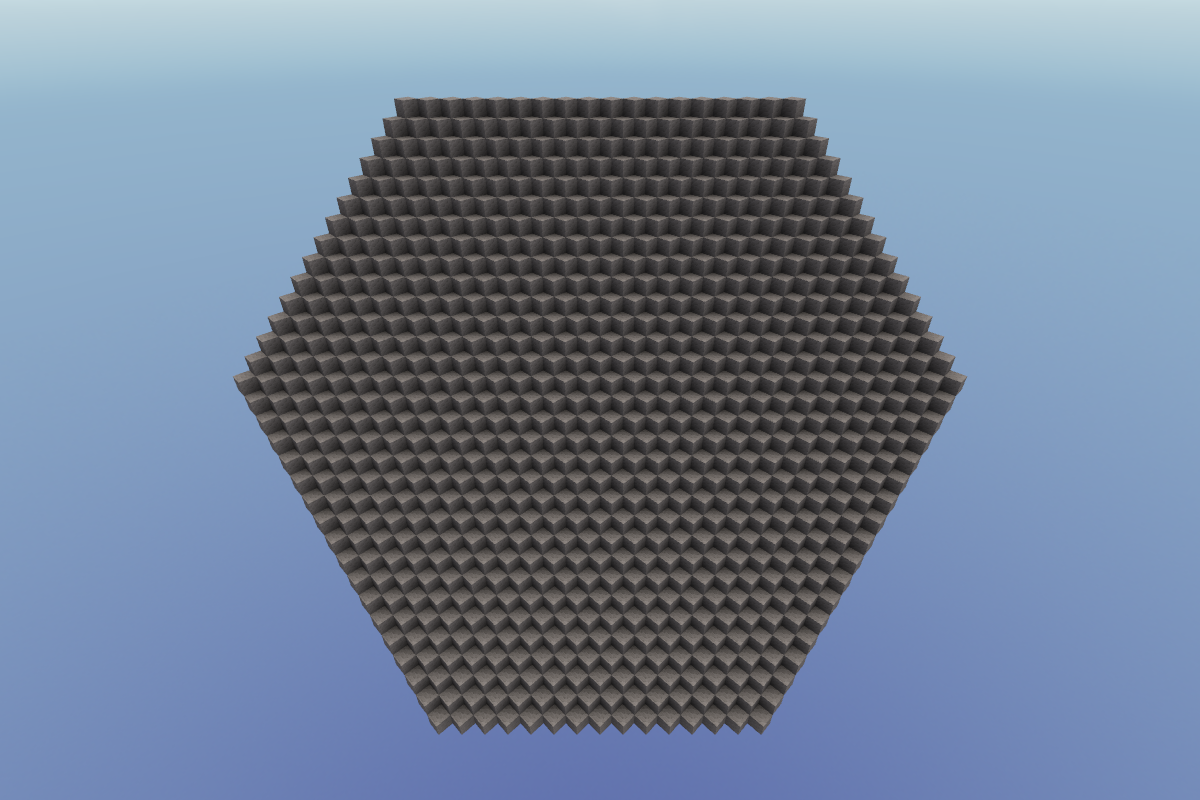
\includegraphics[width=.8\textwidth]{fps-hexagon.png}
	\caption[Bildschirmfoto der Blockformation in Szenario 1 der Performanceanalyse.]{Bildschirmfoto der Blockformation in Szenario 1. Die Blöcke bilden ein stilisiertes Hexagon. Es ist \emph{nicht} gleichseitig. Die Formation ermöglicht den Blick auf je drei Seiten jedes Blocks und besteht aus 766 Blöcken.}\label{fig:hexagon}
\end{figure}
Die Anordnung der Blöcke in Szenario 1 ist in Abbildung~\ref{fig:hexagon} dargestellt. Wie in der Abbildung bei genauem Hinsehen zu erkennen ist, sind von jedem Block drei Seiten sichtbar. Dadurch lässt sich die genaue Anzahl der Elemente bestimmen, die gezeichnet werden, und die Gesamtzahl der gezeichneten Polygone\footnote{In der Blocklib besteht jedes gezeichnete Element aus Dreiecken oder aus Rechtecken, zusammenfassend werden diese als Polygone bezeichnet. Die meisten Elemente in der Welt werden als Dreiecke gezeichnet, die Elemente der graphischen Oberfläche nutzen Rechtecke. Jede Seite eines Blocks setzt sich aus zwei Dreiecken zusammen. Siehe dazu auch Abbildung~\vref{fig:cube}.} für dieses Szenario genau berechnen. Jeden Frame müssen genau $766\cdot3\cdot2 + 3\cdot2-1 = 4596 +5 = 4601$ Polygone gezeichnet werden. Die $5$ zusätzlichen Polygone stammen von der \emph{Skybox}, einem großen Würfel um die Spielwelt herum, der eine Himmelstextur zeigt. Eines der Dreiecke der drei Seiten der Skybox ist außerhalb des Sichtfelds. Daher müssen nur $5$ Polygone hinzugezählt werden.


\paragraph{\ac{fps}} Abbildung~\ref{fig:seed-0-hexagon-fps} zeigt den Verlauf der \si{\fps}. Die Framerate unter \sysA{} ist durchschnittlich \SI{337}{\fps} und unter \sysB{} \SI{1133}{\fps}. Das ist ein Zuwachs von \SI{236}{\percent}. Unter \sysA{} ist der Start der Blocklib schneller. Hier werden Frames nach 11 Sekunden erzeugt, in \sysB{} nach 13 Sekunden. \sysB{} benötigt für den Start also \SI{21}{\percent} mehr Zeit. Über die Zeit hinweg bleiben die Frameraten beider Systeme in etwa konstant.
\begin{figure}[!htbp]
	\settowidth\mytemp{1,}
	\fpsplot[ytick={0,200,...,1200},height=5cm,ymax=1200,y label style={at={(ticklabel cs:.5,-\mytemp)}}]{seed-0-hexagon}
	\caption{Graph des Verlaufs der Framerate in Szenario 1: Hexagon.}\label{fig:seed-0-hexagon-fps}
\end{figure}


\paragraph{\ac{cpu}} Der Verlauf der Auslastung der \ac{cpu} durch die Blocklib ist in Abbildung~\ref{fig:seed-0-hexagon-cpu} zu sehen. Beide Systeme zeigen hier eine Spitze in der Last beim Start der Blocklib. In \sysA{} ist die maximale Auslastung von \SI{47}{\percent} nach 11 Sekunden erreicht, \sysB{} erreicht eine Auslastung von \SI{42}{\percent} nach 15 Sekunden. Die maximale Last ist bei \sysB{} \SI{11}{\percent} niedriger als bei \sysA{}. Die durchschnittliche Auslastung in der Hauptphase ist in \sysB{} mit einem Wert von \SI{18}{\percent} um \SI{38}{\percent} höher als in \sysB{} mit durchschnittlich \SI{13}{\percent}. Nach den anfänglichen Spitzen ist die Auslastung in \sysA{} ab Sekunde 15 und in \sysB{} ab Sekunde 17 in etwa konstant.
\begin{figure}[!htbp]
	\cpuplot{seed-0-hexagon}
	\caption[Graph des Verlaufs der \glsentryshort{cpu}-Auslastung in Szenario 1: Hexagon.]{Graph des Verlaufs der \ac{cpu}-Auslastung in Szenario 1: Hexagon.}\label{fig:seed-0-hexagon-cpu}
\end{figure}


\paragraph{\ac{gpu}} Der in Abbildung~\ref{fig:seed-0-hexagon-gpu} dargestellte Graph beschreibt die Last der \ac{gpu} im zeitlichen Verlauf. Da für diese Messungen ein externer Profiler genutzt wird, kann die Auslastung der \ac{gpu} über die gesamte Messdauer hinweg ermittelt werden. Die Daten zu Beginn und zum Ende der Messung sind allerdings mit Vorsicht zu betrachten. So ist die Auslastung bei Sekunde $0$ der Messung nicht der Blocklib selbst zuzuordnen und zum Ende der Messung kann der Abfall der Last nach dem Beenden der Blocklib beobachtet werden. 
\begin{figure}[!htbp]
	\gpuplot{seed-0-hexagon}
	\caption[Graph des Verlaufs der \glsentryshort{gpu}-Auslastung in Szenario 1: Hexagon.]{Graph des Verlaufs der \ac{gpu}-Auslastung in Szenario 1: Hexagon.}\label{fig:seed-0-hexagon-gpu}
\end{figure}

Da der \ac{gpu}-Profiler manuell gestartet werden muss, lassen sich die Auslastungswerte zu Beginn der Messung nicht gesichert vergleichen. Da der steile Abfall der Last nach dem Beenden der Blocklib bei beiden Systemen gleichzeitig ist, kann aber angenommen werden, dass zumindest grobe Trends zeitlich vergleichbar sind.

Auch in der Auslastung der \ac{gpu} ist zu erkennen, dass der Start der Blocklib mit \sysA{} schneller als mit \sysB{} abläuft. Während in \sysA{} bereits nach 7 Sekunden eine Auslastungsspitze von \SI{27}{\percent} gemessen wird, ist der erste markante Anstieg der Last (auf \SI{27}{\percent}) in \sysB{}  erst nach 12 Sekunden zu sehen. Die durchschnittliche Auslastung ist in beiden Systemen mit \SI{38}{\percent} in \sysA{} und \SI{36}{\percent} in \sysB{} fast identisch (Anstieg von \SI{1}{\percent} in \sysB{}). Während in \sysB{} nach 20 Sekunden und dem Abschluss der Startphase die Last fast konstant knapp unter \SI{40}{\percent} liegt, schwankt die Auslastung in \sysA{} lange zwischen \SI{30}{\percent} und \SI{40}{\percent}, bis sie schließlich nach etwa 50 Sekunden ebenfalls konstant bei knapp \SI{40}{\percent} liegt.

\begin{figure}[!htbp]
	\memplot[xticklabels={,,},xlabel={}]{seed-0-hexagon-multi-mem.csv}{\sysA}
	\\\memplot{seed-0-hexagon-multi-mem.csv}{\sysB}
	\caption{Graph des Verlaufs der Speichernutzung in Szenario 1: Hexagon.}\label{fig:seed-0-hexagon-mem}
\end{figure} 
\paragraph{\ac{ram}} Betrachtet man den in Abbildung~\ref{fig:seed-0-hexagon-mem} gezeigten Vergleich der Speichernutzung zwischen \sysA{} und \sysB{}, lässt sich erkennen, dass \sysB{} sowohl während des Starts der Blocklib als auch allgemein mehr Speicher benötigt als \sysA{}. Der gelbe Bereich zeigt den von Java insgesamt angeforderten Speicher. Zu Beginn ist das bei \sysB{} \SI{1730}{\mega\byte} und während des Großteils der Messung \SI{947}{\mega\byte}. \sysA{} benötigt die ersten 37 Sekunden \SI{644}{\mega\byte} Speicher, was sich bis zum Ende der Messung auf \SI{382}{\mega\byte} verringert. Durchschnittlich benötigt \sysB{} mit \SI{947}{\mega\byte} \SI{64}{\percent} mehr Speicher als \sysA{} mit durchschnittlich \SI{576}{\mega\byte} Speicherbedarf.

Der rote Bereich zeigt den Speicherverbrauch kurzlebiger Objekte an. Die Speichermenge dieser Objekte wird \emph{Eden(-Space)} genannt. In \sysB{} steigt die Menge der neu erzeugten Objekte deutlich schneller an als in \sysA{}. Damit einher geht auch die Anzahl der durchgeführten \emph{Garbage-Collections}\footnote{Wird ein Objekt in Java nicht mehr gebraucht, kann der Speicher wieder freigegeben werden. Das passiert automatisch durch den sogenannten Garbage-Collector. Dieser wird nicht immer sofort tätig, sondern nur zu bestimmten Situationen, insbesondere dann, wenn die freie Speichermenge zuneige geht.}. Die Spitzen in den roten Graphen markieren Zeiten zu denen der Garbage-Collector aktiv geworden ist. In \sysA{} gibt es über die gesamte Messdauer 13 Garbage-Collections, in \sysB{} sind es 21. Damit lässt sich abschätzen, dass \sysB{} kontinuierlich etwa \SI{61}{\percent} schneller Speicher mit neu erzeugten, kurzlebigen Objekten belegt als \sysA{}. Hier ist allerdings nicht berücksichtigt, dass \sysB{} mehr Speicher belegt, und somit weniger Garbage-Collections benötigt, wenn die Erzeugungsraten gleich sind. Berechnet man die mittlere Steigung der positiven Anstiege des roten Graphen, kann man ermitteln, wie viel Speicher pro Sekunde für die Erzeugung neuer Objekte genutzt wird. \sysA{} verbraucht \SI{70}{\mega\byte\per\second}, \sysB{} respektive \SI{274}{\mega\byte\per\second}. Das ist ein Anstieg von \SI{291}{\percent}, was deutlich mehr als die geschätzten \SI{61}{\percent} ist.

Der Speicherbedarf der langlebigen Objekte, der auch \emph{Tenured(-Space)} genannt werden, wird in der Abbildung durch den blauen Graphen dargestellt. In beiden Systemen ändert sich dieser Speicherbedarf deutlich weniger als Eden, das ist allerdings nicht vollständig aussagekräftig, da der Garbage-Collector den Tenured-Bereich seltener bereinigt als den Eden-Bereich. Während der Tenured-Speicherbedarf in \sysB{} in der Hauptphase konstant bleibt, verringert er sich in \sysA{}. 